\subsection{Application Installation} \label{subsection:android-install}
Before running an application, the \gls{apk} containing the code, has to be installed.
The installation consists of two major steps.
The first step is primarily about verification, while the second step is the bytecode optimization and, in case of \gls{art}, the code compilation (see figure~\ref{fig:install}).
The differences will be explained in the following subsections.
\newline
Before initiating the installation, the \gls{apk} is checked for its integrity and authenticity.
The \textit{META-INF} folder contains the necessary files for performing the signature verification process.
The three files are the \textit{MANIFEST.MF}, the \textit{MANIFEST.SF} und the \textit{CERT.RSA}.
The manifest, \textit{MANIFEST.MF}, contains the name and the digest of each file inside the \gls{apk}, e.g. \textit{classes.dex} and its signature.
The the signature file, \textit{MANIFEST.MF} which is used for the code signing.
It is similar to the manifest and contains the SHA1 digest of the manifest and the digests of each entry inside the manifest.
The \textit{CERT.RSA} is the digital signature, called signature block, which is used to sign the files.
While the manifest files are used to detect tampering while the digital signature is used to identify the code signer.
In order to apply updates, the old and the new \gls{apk} need to have the same package name and code signer.
Since Android allows self-signed certificates, no connection of whether the \gls{apk} was signed by the right person nor whether the application is allowed to be installed can be closed from the digital signature
\cite{codeSigning} \cite{androidSigning}
\newline
The installation can be performed in two ways depending on the runtime of the Android \gls{os}.
For the \gls{dvm}, optimisation is applied to the \textit{classes.dex} file and the corresponding \gls{odex} file is generated and moved to the Dalvik cache.
As a reminder, the \gls{odex} is an optimization tailored to the specific architecture of the device for the best performance due to the the high diversity of Android hardware and their different processors.
This is done once on installation.
Future application starts will execute the \gls{odex} file instead of the the \gls{dex} file.
This preprocessed version of the application has an improved startup time. \cite{kovachevaMaster}
\newline
Currently, the Android runtime of choice is \gls{art}.
For this runtime, the second step is more complex since the bytecode has to be compiled an additional time.
This will be explained closer in section~\ref{subsection:android-art}.
\newline
After the bytecode is optimized respectively compiled, the application can be run.
\newline
\begin{figure}[h]
    \centering
    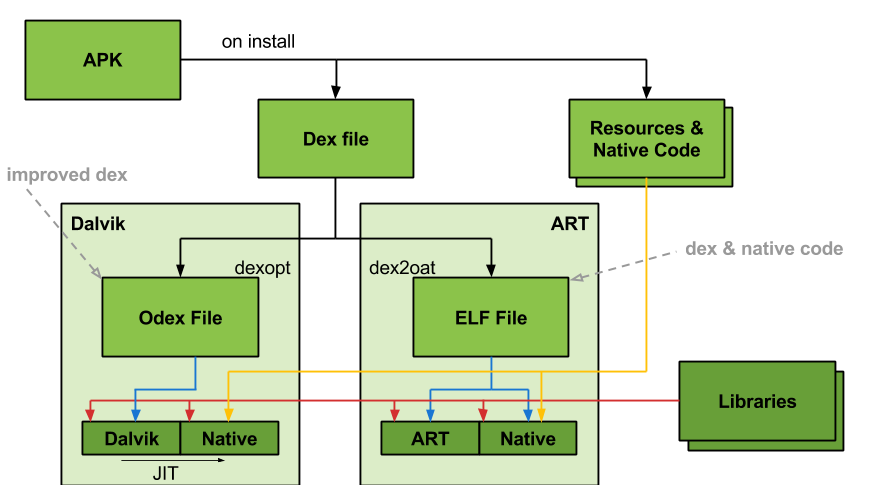
\includegraphics[width=0.8\textwidth]{data/install.png}
    \caption{Installing an \gls{apk} on a device \cite{googleIOArt}}
    \label{fig:install}
\end{figure}
When the application is run on the device, Android creates a sandboxed environment for application only.
This means each process an own \gls{vm} and separate user ID and cannot access any resources except their own. \cite{developerFundamentals}
